\section{Neighbor Discovery Protocol}
\label{sec:technique}
 
As noted earlier, co-residence detection scales well when co-residing instances
on each server communicate among themselves and discover each other.  Assuming
that the instances have unique IDs, this requires the co-resided instances to
exchange these (integer) IDs with each other using the memory bus channel as a
transmission medium. In this section, we present a communication protocol that
the co-resided instances can use to achieve communication in a fast and reliable
way. We first discuss the challenges we faced in making the channel reliable
before examining the protocol itself.

\begin{algorithm}[!t]
\caption{Writing 1-bit from the sender}
\label{alg:sender}
\begin{algorithmic}
\STATE $now \leftarrow  time.now()$
\STATE $end \leftarrow now + sampling\_duration$
\STATE $address \leftarrow cache\_line\_boundary-2$
\WHILE{$now < end$}
    \STATE $\_\_ATOMIC\_FETCH\_ADD(address)$
    \STATE $now \leftarrow  time.now()$
\ENDWHILE
\end{algorithmic}
\end{algorithm}

\subsection{Reliable Transmission}
Senders and receivers can reliably communicate 0-bits and 1-bits by causing
contention on the memory busy.  Consider the simple scenario where there is one
sender and one receiver instance on a machine, and the sender has a set of bits
that it needs to communicate with the receiver on the memory bus covert channel.
To communicate a 1-bit, the sender instance causes contention on the memory busy
by locking it using the special memory locking operations (discussed in
section~\ref{sec:background:membus}). The receiver would then sample the memory
bus for contention, inferring whether the communication is a 1-bit (when
contention is observed) or a 0-bit (when contention is not observed).
Pseudo-code for the sender instance is shown in Algorithm~\ref{alg:sender}.

\subsubsection{Sensing contention} 
There are two ways in which the receivers could detect memory bus contention.
When the memory bus is locked, any non-cached memory accesses will queue and
therefore see higher latencies. The receiver can then continually make un-cached
memory accesses (referred to as the \textit{memory probing} receiver in previous
literature~\cite{varadarajan2015}) and observe a spike in their latencies to
detect contention.  The receiver can also detect memory bus contention by using
the same memory locking operations as the sender (referred to as \textit{memory
locking} receiver) to probe the memory bus. Since only one processor core can
lock the memory bus at a given time, any other concurrent locking operation will
see higher latency. 

Thought two methods exist for detecting memory bus contention, we decide to use
the memory locking receiver for our experiments. Previous
studies\cite{wuusenix2012,varadarajan2015} have established that both memory
probing and memory locking receivers experience significant latency overhead
during memory bus contention, making them both avenues for sensing the
covert-channel. Memory probing involves regular (un-cached) memory accesses,
which is universal, unlike the locking operations which are rarely used, if at
all, by standard applications. This makes memory probing the only viable option
for \textbf{non-cooperative} co-residence detection, where victims are not under
attacker's control and cannot be assumed to perform locking operations.
Furthermore, memory probing can be done on multiple receivers constantly without
affecting each other (due to the high memory bandwidth), which prevents noise in
measurements.  This is an important attribute, as memory locking receivers must
contend with this noise. However, bypassing multi-levels of caches in today's
servers to perform memory accesses with reliable consistency is a challenging
task \todo{cite some papers}. Even with a reliable cache-bypassing technique,
the variety of cache architectures and sizes that we encounter on different
clouds would make tuning the technique to suit these architectures an arduous
task while reducing the applicability of our overall co-residence detection
mechanism.  Thus, we decide to use the memory locking receiver.


\begin{algorithm}[!t]
\caption{Reading a bit in the receiver}
\label{alg:receiver}
\begin{algorithmic}[1]
\STATE $now \leftarrow  time.now()$
\STATE $end \leftarrow now + sampling\_duration$
\STATE $sampling\_rate \leftarrow num\_samples / sampling\_duration$
\STATE $address \leftarrow cache\_line\_boundary-2$
\STATE $samples \leftarrow \{\} $
\WHILE{$now < end$}
    \STATE $before \leftarrow RDTSC()$
    \STATE $\_\_ATOMIC\_FETCH\_ADD(address)$
    \STATE $after \leftarrow RDTSC()$
    \STATE $samples \leftarrow samples \cup \{(after-before)\}$
    \STATE \textbf{wait until} $NEXT\_POISSON(sampling\_rate)$
    \STATE $now \leftarrow  time.now()$
\ENDWHILE
\STATE $ks\_val \leftarrow KOLMOGOROV\_SMIRINOV(samples, baseline)$
\STATE \textbf{return} $ks\_val < ksvalue\_threshold$
\end{algorithmic}
\end{algorithm}


\subsubsection{Sampling frequency}
Ideally, a memory locking receiver would loop locking operations and determine
contention in real-time by identifying a decrease in the moving average of the
number of operations. Note that, in this case, there is essentially no
difference between the sender and receiver (i.e., both continually issue locking
operations) except that the receiver is taking measurements. This is adequate
when there is a single sender and receiver~\cite{varadarajan2015}, but when
there are multiple receivers, the mere act of sensing the channel by one
receiver causes contention and other receivers cannot differentiate between a
silent (0-bit) and a locking (1-bit) sender. To avoid this, we space the
sampling of memory bus such that no two receivers would sample the bus at the
same time, with high probability.  We achieve this by using large intervals
between successive samples and a poisson-sampling to prevent time-locking of
receivers. We determined that a millisecond poisson gap between samples is
reasonable to minimize noise due to collisions in receiver
sampling~\ref{fig:membus_clouds}, assuming ten co-resided receivers and sampling
takes a few microseconds each time.

\subsubsection{Sampling duration}
\label{sec:method:samplingdur}
A receiver can confirm contention with high confidence with only a few samples,
assuming that the sender is actively causing contention on the memory bus and
the receiver is constantly sampling the memory bus throughout the sampling
duration.  However, in practice, the time-sharing of processors produces
difficulties.  The sender is not continually causing contention, and neither is
the receiver sensing it, as they are context-switched by the scheduler to run
other processes.  Assuming that the sender and receiver are running on different
cores, the amount of time they are actively communicating depends on the
proportion of time they are allocated on each core and how they are scheduled. 

To illustrate such behavior, we run a sender-receiver pair using the
Lambdas\cite{awslambda} of various sizes on AWS, and compare the distribution of
latencies seen by the receiver during the contention in each case. Figure
\ref{fig:context_switching} shows that the much smaller 128 MB lambdas (which
probably share a CPU core and are thus context-switched) exhibit less active
communication than the bigger 3 GB lambdas (which may run on dedicated cores).
This means that smaller instances that tend to share processor cores with a lot
of other instances may need to pause for more time and collect more samples to
make up for lost communication due to scheduling.
% Since the typical scheduling quantum is on the order of milliseconds, they 
% will need at least a second?


\begin{figure}[!t]
  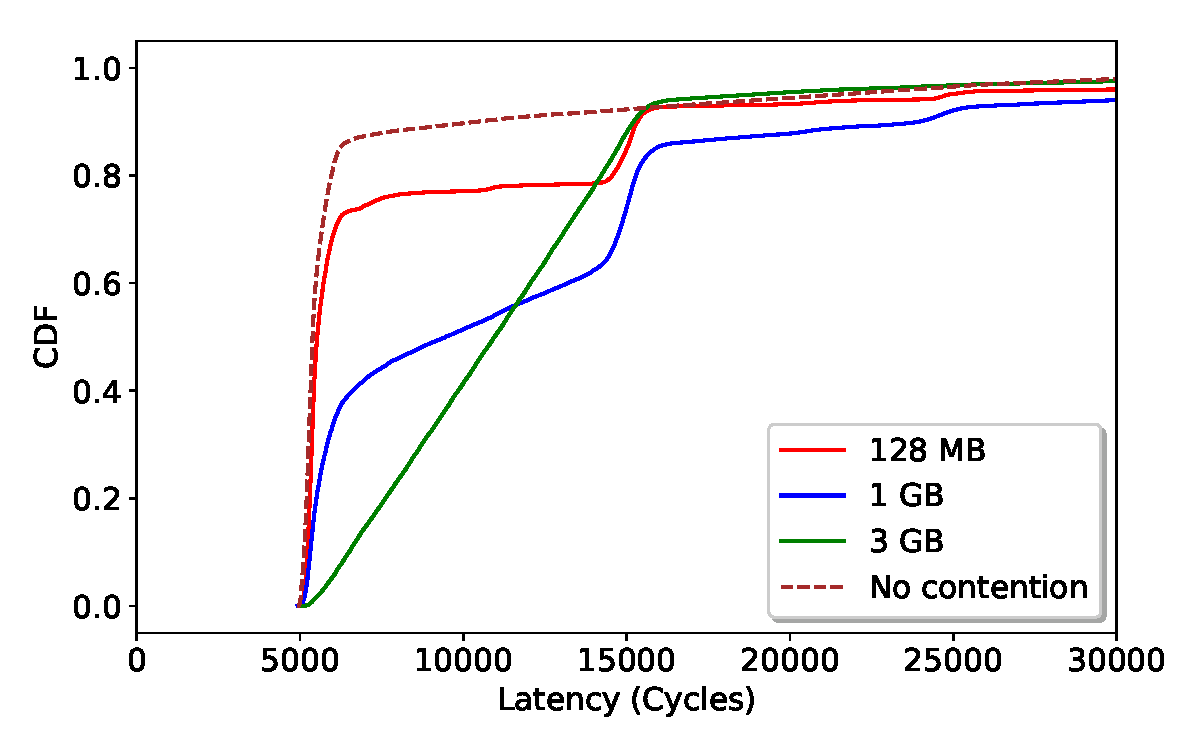
\includegraphics[width=.99\linewidth]{fig/lambda_sched_effect.pdf}
  \caption{Shows CDF of latencies observed by 128 MB, 1 GB and 3 GB Lambdas during 
  contention. The 128 MB lambda pair sees less contention due to more context switching, 
  whereas the 1 GB and 3 GB lambdas see progressively more contention compared to baseline 
  which we attribute to their relative stability on the underlying physical cores. 
\label{fig:context_switching}}
\end{figure}

\subsubsection{Overcoming noise} 
\label{sec:method:noise}
Along with context switching and sensing noise, there are other imperfections in
measurement apparatus that cause (minor) noise. For example, we use the
difference in \amirian{is this the first time we mention RDTSC? do we need to
define it for a community liek this?}RDTSC timer readings before and after the
locking operation to measure its\amirian{what is its in this case?} latency in
cycles. If the receiver process is context-switched in between the timer
readings (e.g., at line 8 in Algorithm \ref{alg:receiver}), the latency measured
from their difference will be orders of magnitude higher as it includes the
waiting time of the receiver process in the scheduler queue - which we believe
is what contributes to the long tail in Figure \ref{fig:context_switching}. To
overcome missed samples and noise, we record hundreds of samples and compare it
to the baseline distribution of latencies sampled without contention. We then
need to compare and differentiate the observed sample of latencies from the
baseline to establish contention. Since we effectively need to compare the
empirical CDFs of the baseline measurements to the contention measurements, we
deicde to use a variant of the two-sample Kolomogorov-Smirinov (KS) test. By
taking the mean of the absolute differences between the empirical CDFs, we can
categorize a KS-value above a certain threshold (KS-threshold) as a 1-bit or a
0-bit.

To determine the threshold, we deploy a large number of lambdas across AWS
regions. Some of these lambdas cause contention (aka senders) while others
observe contention by collecting samples of latencies (aka receivers). Each of
the samples may or may not have observed contention depending on whether the
receiver was co-located with a sender lambda (an unknown at this point). We then
calculate the KS-value for each sample against the baseline and plot a CDF of
these values for lambdas of different sizes in Figure \ref{fig:ks_values}.
Ideally, we expect a bi-modal distribution (stepped CDF) with the lower and
upper peaks corresponding to samples that have not and have seen contention
respectively, and a big gap between the two (long step). Fortunately, we examine
this differentiation with larger lambda sizes (which allows us to choose a clear
threshold), but we do not examine a clear differentiation with smaller lambdas,
where scheduling instability causes lossy communication (discussed in
\ref{sec:method:samplingdur}).  This trend also reflects in the reliability of
our technique across various lambda sizes, as we will show in our evaluation.
Based on the plot, we picked a KS-threshold at 3.0 which seems to be constant
across AWS regions, suggesting that this is a platform constant.

We present the pseudo-code of a receiver lambda in Algorithm~\ref{alg:receiver},
which includes all the limitations discussed thus far.\amirian{I'm not a huge
fan of this sentence...need to find a way to rework}

\subsubsection{Clock synchronization} 
Since communicating each bit of information takes time (i.e., receiver sampling
duration), our algorithm requires synchronizing sender and receiver at the start
of each bit. In traditional analog channels, this is achieved either using a
separate clock signal or a self-clocking signal encoding. For example,
\cite{whispers} uses differential Manchester encoding for clock synchronization
for the memory bus covert channel.  Self-clocking encodings  become much
trickier (\ques{why?}) when there are multiple senders and receivers. In this
work, we use the system clock for synchronizing communication.
All the instances involved in the communication would be running on the same
physical server and so they share the server's clock.  The system clock on AWS
lambdas, for example, is precise up to nanoseconds with a sub-microsecond drift
between different lambdas running on the same server, which is accurate
enough as we only work in the millisecond regime due to sampling noise
constraints\amirian{is there some sort of citation for this?}
% this would limit application to VMs.. but containers are probably okay..


\begin{figure}[!t]
  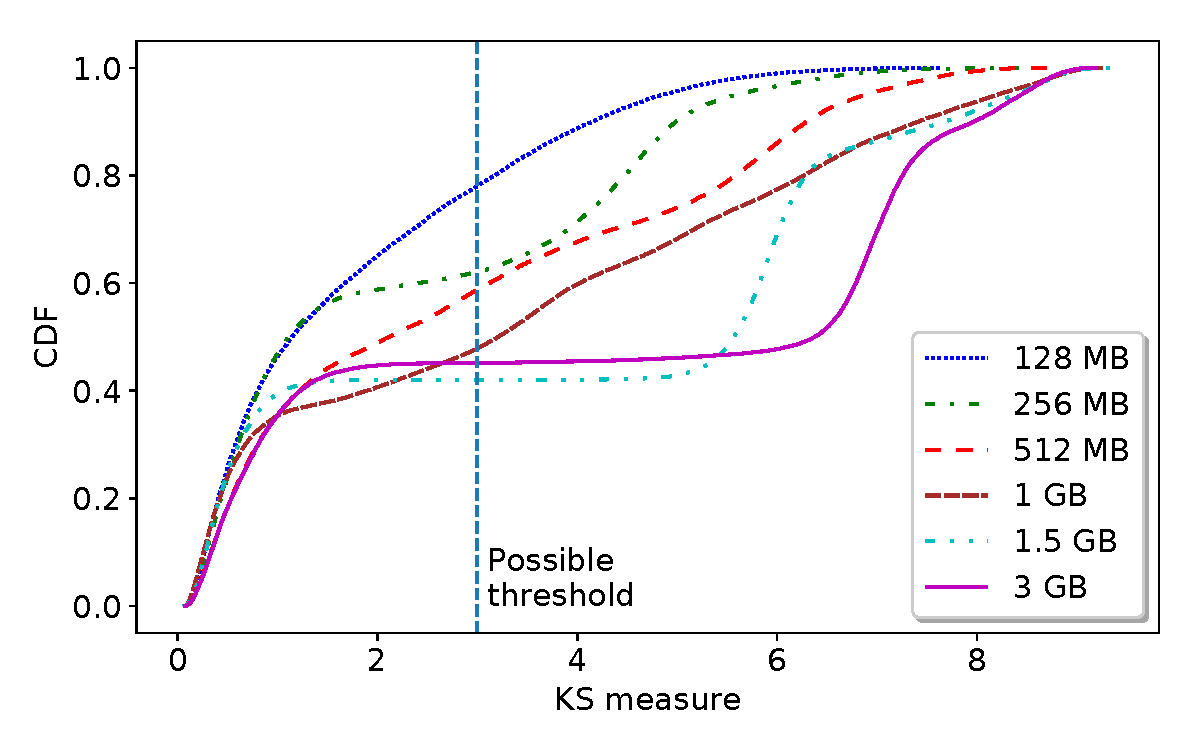
\includegraphics[width=.99\linewidth]{fig/ksvalues.pdf}
  \caption{Shows CDF of KS values observed for various lambda sizes. A bimodal distribution 
  with longer step lets us pick a KS-threshold that enables our technique to differentiate 
  between 0-bit and 1-bit with high confidence. 
\label{fig:ks_values}}
\end{figure}

\subsection{Protocol}
\label{sec:protocol}
In the preceeding section, we discussed a communication channel with
synchronized time slots. In each time slot, an instance can reliably send
(broadcast) or receive (listen) a bit by causing or sensing for contention.
Given that there are multiple instances that may want to broadcast information
on the channel, we next must determine which instance broadcasts first, to avoid
collisions.  Traditional channels like Ethernet or Wireless detect and avoid
collisions by employing a random \amirian{colloquial?}"back-off" mechanism.
This type of mechanism will be challenging to implement in methodology for two
reasons.  First, lambda instances do not have the capability of sensing the
channel while sending a bit, which is required for detecting collisions;
instances can either cause contention or sense it, but not both. Note that
senders do experience a higher latency for locking operations when other senders
are simultaneously causing contention. However, reliably judging this higher
latency requires each sender to already have calculated a baseline of latencies
without collisions\amirian{chicken and egg is a bit too colloquial...need to
figure out how to communicate this thought better}. Second, even implementing a
random "back-off" mechanism will introduce significant overhead before any
meaningful communication occurs. This overhead will also increase as the number
of instances involved increases. Since each time slot takes up to 1 second, the
additional overhead can be detrimental to the efficacy of the communication
channel.
\anil{get information theoretic bounds on the capacity of our channel?}


\begin{algorithm}[!t]
\caption{ID exchange protocol \todo{Improve pseudo-code}}
\label{alg:protcol}
\begin{algorithmic}[1]
\STATE $sync\_point \leftarrow$ {Start time for all instances}
\STATE $ID \leftarrow$ {Instance ID}
\STATE $N \leftarrow$ {Number of bits in ID}
\STATE $advertising \leftarrow TRUE$
\STATE $instances \leftarrow \{\} $
\STATE $WAIT\_TILL(sync\_point)$
\WHILE{$id\_read$}
    \STATE $slots \leftarrow 0$
    \STATE $id\_read \leftarrow 0$
    \STATE $participating \leftarrow advertising$
    \WHILE{$slots < N$}
        \STATE $bit \leftarrow$ {$slots^{th}$ most significant bit of ID}
        \IF{$participating$ \textbf{and} $bit$}
            \STATE $WRITE\_BIT()$               (Alg. \ref{alg:sender})
            \STATE $bit\_read \leftarrow 1$
        \ELSE
            \STATE $bit\_read \leftarrow READ\_BIT()$       (Alg. \ref{alg:receiver})
            \IF{$bit\_read$}
                \STATE $participating \leftarrow FALSE$
            \ENDIF
        \ENDIF
        \STATE $id\_read \leftarrow 2 * id\_read + bit\_read$
        \STATE $slots \leftarrow slots + 1$
    \ENDWHILE
    \IF{$id\_read = ID$}
        \STATE $advertising \leftarrow FALSE$
    \ENDIF
    \STATE $instances \leftarrow instances \cup \{id\_read\}$
\ENDWHILE
\STATE \textbf{return} $instances$
\end{algorithmic}
\end{algorithm}

\amirian{I think in general we need a bit more sign-posting to guide the reader.
I will think about this a bit more}.
However, a communication channel for lambda co-residence detection need not be
general and expressive\amirian{why?}.  Thus, we assume that each instance
involved has a unique fixed-length (say \emph{n}) bit-string corresponding to
its ID that must be communicated.  As such, we propose a communication protocol
that exchanges these bit-strings while allowing for collisions. We divide the
running time of the protocol into phases, with each phase executing for an
interval of \textit{n} bit-slots. Each phase has a set of participating
instances, which in the first phase would be all of the co-located instances. In
each bit-slot \textit{k} of \textit{n} slots in a phase, every participating
instance broadcasts a bit if the $k^{th}$ bit of its bit-string (ID) is 1,
otherwise it listens for a 0 or 1. If an instance senses a 1 while listening, it
stops participating, and listens for the rest of the phase. Thus, only the
instances with the highest ID among the initial set of participating lambdas
continues broadcasting until the end of the protocol, effectively advertising
its full ID to the rest of the (now listening) lambdas). In the next cycle, the
lambda with the previously highest ID now only listens, allowing the next
highest instance to advertise its ID, and so on.  Since the IDs are unique,
there will always be only one instance that broadcasts in every phase. The
protocol ends after \textit{x} phases (where \textit{x} is number of co-located
instances), when none of the instances broadcast for \textit{n} consecutive
bit-slots.  A pseudo-code of the protocol is provided in Algorithm
\ref{alg:protcol}. Note that the protocol itself is channel-agnostic and can be
extended for other (future) covert channels with similar channel properties.

% Figure moved here for formatting
\begin{figure}[!t]
  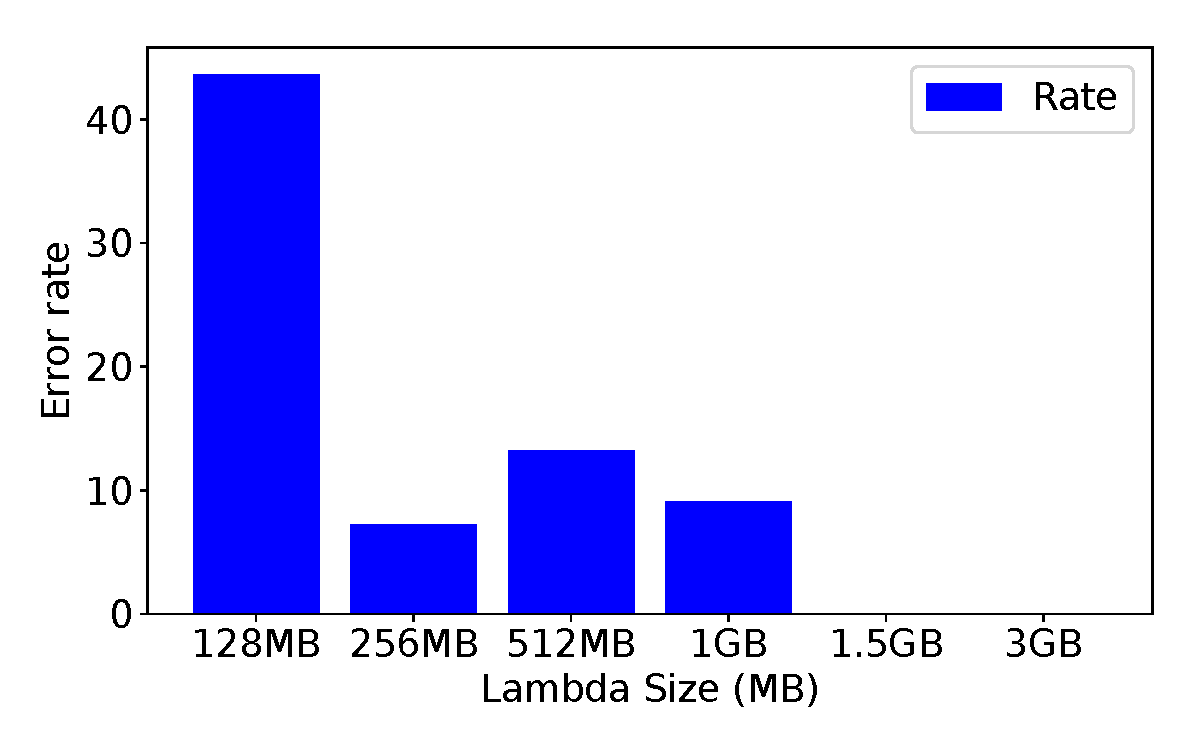
\includegraphics[width=.99\linewidth]{fig/errorrates.pdf}
  \caption{Shows the error rate (as a fraction of 1000 lambdas deployed) for different lambda sizes in AWS Middle-East region. 
\label{fig:errorrates}}
\end{figure}

\subsubsection{Complexity}
\label{sec:protocol:complexity}
Assuming \textit{N} total deployed instances to the cloud, the bit-string needs
to be $\log_2N$ bits to uniquely identify each instance. If a maximum \textit{K}
of those instances are launched on the same server, the protocol executes for
\textit{K} phases of $\log_2N$ bit-slots each, taking $(K+1)*\log_2N$ bit-slots
for the whole thing. For example, assuming 10,000 deployed lambdas and a maximum
of 10 co-located instances on each server, the entire  co-residence detection
requires around 4 minutes to fully execute (with 1-second time slots).  In fact,
it is not necessary to run the protocol for all \textit{K} phases. After the
first round, all the co-located instances would know one of their neighbors.
\amirian{confused about this sentence} Instances can exchange the globally
unique IDs offline (through the network) to determine the rest of their
neighbors.  This simplification removes the dependency on number of co-located
instances (\textit{K}) and decreases the complexity to $O(\log_2N)$, allowing
the entire protocol to finish within a minute instead of four.


% \subsubsection{Limitations}
% challenge with same core scheduling. - write a list of drawbacks?
% this could be overcome by getting 
% redundant info and constructing 
% the graph
